% !TEX root = ../notes_unsupervisedlearning.tex
% Chapter 4: Density and Graph-Based Clustering
%%%%%%%%%%%%%%%%%%%%%%%%%%%%%%%%%%%%%%%%%%%%%%%%%%%%%%%%%%%%%%%%%%%%%%

\chapter{Density and Graph-Based Clustering}\index{DBSCAN}\index{spectral clustering}
\newthought{It is all about that space, about that space.}

% ==============================================================================================
% BLOCK 1: INTRODUCTION
% ==============================================================================================

\newthought{The Why}\index{density-based clustering}

Hierarchical clustering gave us every scale of structure at once, but it never learned to say 
``this point belongs to nothing.''
Every point, no matter how isolated, is absorbed into some cluster at the final merge.
Real data contains noise: GPS measurements with dropouts, sensor readings during interference, survey responses that are genuine outliers.
A method that must absorb every point will misrepresent noise as structure.

As we look at a map of taxi pickup locations, we immediately see dense corridors of activity and a handful of isolated points far from any group.
Our eye does not force those outliers into the nearest cluster; it marks them as noise and focuses on where the true structure lies.
The process of finding regions of density is called density-based clustering.

\newthought{Density-based clustering} reframes the question entirely.
Instead of asking how far a point is from a centroid or a neighbouring cluster, it asks how densely packed the neighbourhood around a point is.
A cluster is a maximal connected region where points are dense; any point in a sparse region is declared noise outright.
Road networks cluster into corridors of taxi GPS traces, not spheres.
Social communities cluster into groups of densely connected users, not groups close to a central member.

\marginnote{\newthought{Two complementary ideas.} Density-based methods (DBSCAN, OPTICS) ask: is this region of space dense enough to be a cluster? Graph-based methods (spectral clustering) ask: is this set of points more connected to each other than to the rest? Both escape the spherical cluster assumption that limits K-Means and hierarchical clustering.}

\newthought{The key insight} is that a cluster need not have a centre.
It needs only a notion of neighbourhood: two points belong to the same cluster if they are close enough, and that closeness can chain through intermediate points.
This lets clusters take arbitrary shapes, detect noise naturally, and avoid committing to $K$ in advance.

\begin{marginfigure}
    \centering
    \begin{tikzpicture}
        \begin{axis}[
            xmin=0, xmax=8, ymin=0, ymax=8,
            width=\marginparwidth, height=\marginparwidth,
            axis line style={draw=none},
            tick style={draw=none},
            xtick=\empty, ytick=\empty,
        ]
        % Dense cluster with epsilon circle
        \draw[black!40, dashed] (axis cs:2,2) circle [radius=1.2];
        \addplot[only marks, mark=*, mark size=2pt, black] coordinates {(2,2)(1.5,2.8)(2.8,1.6)(1.8,1.3)};
        % Noise point far away
        \addplot[only marks, mark=*, mark size=2pt, black!30] coordinates {(6.5,6.5)};
        \draw[black!30, dashed] (axis cs:6.5,6.5) circle [radius=1.2];
        \node[font=\tiny, anchor=north] at (axis cs:2,0.9) {cluster};
        \node[font=\tiny, anchor=south] at (axis cs:6.5,7.7) {noise};
        \end{axis}
    \end{tikzpicture}
    \caption{A dense cluster (left) where points share a neighbourhood, and an isolated noise point (right) with no companions within $\varepsilon$. \textit{Density, not distance to a centre, determines membership.}}
\end{marginfigure}

\marginnote{\newthought{No centroid required.} A density-based cluster is a region, not a mean. Its shape is implicit in the data; nothing forces it to be convex or spherical. This assumption-free view is both the strength of density-based methods and, as we will see, the source of their own limitations.}

\newthought{In order to move from pairwise distances to density-aware clusters} we have good reason to find ways to,
\begin{itemize}
    \item define what it means for a region of space to be \emph{dense}, making the notion of a cluster boundary parameter-driven rather than geometrically fixed.
    \item propagate cluster membership through chains of close points, so that arbitrarily shaped clusters emerge from local density alone.
    \item handle graph structure directly, so that connectivity rather than distance governs which points belong together.
\end{itemize}

\newpage
\subsection{Hands On Experience}

\newthought{Consider} the same six canonical points, now with a seventh point $x_7{=}(4,5)$ placed between the two natural groups.

\begin{figure}
\centering
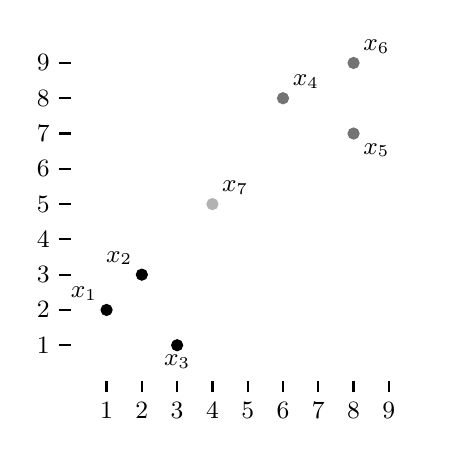
\begin{tikzpicture}[scale=1]
    \begin{axis}[
        xmin=0, xmax=10,
        ymin=0, ymax=10,
        width=0.5\textwidth,
        height=0.5\textwidth,
        axis line style={draw=none},
        tick style={black, thick},
        xtick={1,2,3,4,5,6,7,8,9},
        ytick={1,2,3,4,5,6,7,8,9},
        xticklabel style={font=\small},
        yticklabel style={font=\small},
        tick align=outside,
        tick pos=left,
    ]
    \addplot[only marks, mark=*, mark size=2pt, black] coordinates {
        (1,2) (2,3) (3,1)
    };
    \addplot[only marks, mark=*, mark size=2pt, black!55] coordinates {
        (6,8) (8,7) (8,9)
    };
    \addplot[only marks, mark=*, mark size=2pt, black!30] coordinates {
        (4,5)
    };
    \node[font=\small, anchor=south east] at (axis cs:1,2) {$x_1$};
    \node[font=\small, anchor=south east] at (axis cs:2,3) {$x_2$};
    \node[font=\small, anchor=north]      at (axis cs:3,1) {$x_3$};
    \node[font=\small, anchor=south west] at (axis cs:6,8) {$x_4$};
    \node[font=\small, anchor=north west] at (axis cs:8,7) {$x_5$};
    \node[font=\small, anchor=south west] at (axis cs:8,9) {$x_6$};
    \node[font=\small, anchor=south west] at (axis cs:4,5) {$x_7$};
    \end{axis}
\end{tikzpicture}
\caption{Six canonical points plus $x_7{=}(4,5)$ sitting between the two natural groups. Which points lie in dense neighbourhoods, and which sits in empty space?}
\label{fig:dbscan_intro_scatter}
\end{figure}

\newthought{Draw a circle} of radius $\varepsilon{=}2.5$ around each point.
Which points have at least two neighbours inside their circle?
Which point has no neighbours at all?
If you were forced to assign $x_7$ to one of the two groups, which would you choose, and would you trust that assignment?

\newthought{Noise seems like the right answer} for $x_7$, but could you argue otherwise?
What would happen if you enlarged $\varepsilon$ to 4.5?
And if every isolated point is noise, is there ever a reason to absorb it into a cluster?

\vspace{2.5em}
\newthought{Without fixed parameters}, there is no single right answer, as a choice of $\varepsilon$ and $\mathrm{minPts}$ for any answer could be engineered.
However, some answers are better than others, and most people agree that $x_7$ is better left as noise than silently forced into whichever group happens to be nearest.

\newthought{The fundamental question} this chapter answers is: how do we formalize the notion of a dense neighbourhood so that cluster membership propagates naturally, noise is identified automatically, and no value of $K$ needs to be chosen in advance?

\marginnote{\newthought{The neighbourhood radius $\varepsilon$} is the distance within which a point looks for companions.
Small $\varepsilon$ finds only very tight clusters and labels most points noise.
Large $\varepsilon$ absorbs everything into one cluster.
The right value lives in between, where the data transitions from dense to sparse.
We will see a principled way to find it using the $k$-distance plot.}

\newthought{Where would you place} the boundary between dense and sparse in this data?
Could you think of a way to read that boundary off the data itself, rather than guessing it?

\newthought{The Learning Objectives} of this lecture:
\begin{itemize}
    \item Understand how DBSCAN defines density through $\varepsilon$-neighbourhoods and minimum point counts, and trace the full clustering of a small dataset by hand.
    \item Apply spectral clustering by constructing the similarity graph, computing the Laplacian, and explaining why the eigenvector embedding separates non-convex clusters.
    \item Identify when density-based and graph-based methods succeed where K-Means and hierarchical clustering fail, and recognise their own failure modes.
\end{itemize}


% ==============================================================================================
% BLOCK 2: MAIN THEORY
% ==============================================================================================

\newpage

\newthought{The DBSCAN Algorithm}\index{DBSCAN}

\newthought{DBSCAN}\index{DBSCAN} (Density-Based Spatial Clustering of Applications with Noise) builds clusters from local density.
Two parameters govern the algorithm: $\varepsilon$ (the neighbourhood radius) and $\mathrm{minPts}$ (the minimum number of points required to form a dense region).

\marginnote{\newthought{DBSCAN.} Introduced by Ester, Kriegel, Sander, and Xu in 1996. One of the most cited clustering algorithms, and a standard benchmark for density-based methods.}

\newthought{Every point is classified} into one of three roles before any cluster is formed.
A point $p$ is a \textbf{core point}\index{core point} if its $\varepsilon$-neighbourhood contains at least $\mathrm{minPts}$ points:
\begin{align*}
    N_\varepsilon(p) &= \{q \in X : d(p,\,q) \leq \varepsilon\} \\[4pt]
    p \text{ is core} &\iff |N_\varepsilon(p)| \geq \mathrm{minPts}
\end{align*}

A point $q$ is a \textbf{border point}\index{border point} if it is not a core point but falls within the $\varepsilon$-neighbourhood of some core point.
A point is \textbf{noise}\index{noise point} if it is neither core nor border.

\marginnote{\newthought{Density reachability} is not symmetric. A border point $q$ is reachable from core point $p$ (because $q \in N_\varepsilon(p)$), but $p$ is not reachable from $q$ (because $q$ is not core). Cluster membership propagates from cores outward, never in reverse.}

\begin{figure}
\centering
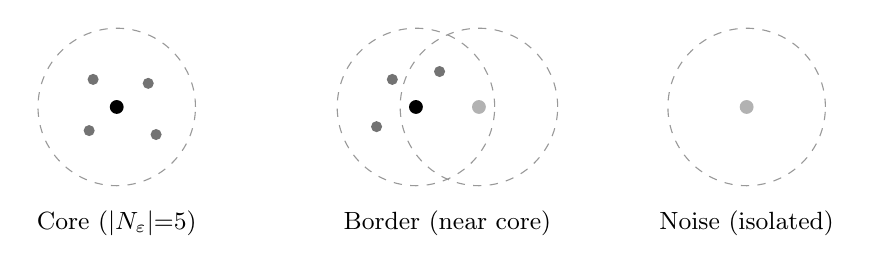
\begin{tikzpicture}
    % Core point
    \draw[black!40, dashed] (0,0) circle (1.0cm);
    \fill[black]    (0,0)         circle (2.5pt);
    \fill[black!55] ( 0.40, 0.30) circle (2pt);
    \fill[black!55] (-0.30, 0.35) circle (2pt);
    \fill[black!55] ( 0.50,-0.35) circle (2pt);
    \fill[black!55] (-0.35,-0.30) circle (2pt);
    \node[font=\small, anchor=north] at (0,-1.2) {Core ($|N_\varepsilon|{=}5$)};

    % Border point (core at 3.8, border at 4.6)
    \draw[black!40, dashed] (3.8,0) circle (1.0cm);
    \draw[black!40, dashed] (4.6,0) circle (1.0cm);
    \fill[black]    (3.8, 0)    circle (2.5pt);
    \fill[black!55] (3.5, 0.35) circle (2pt);
    \fill[black!55] (3.3,-0.25) circle (2pt);
    \fill[black!55] (4.1, 0.45) circle (2pt);
    \fill[black!30] (4.6, 0)    circle (2.5pt);
    \node[font=\small, anchor=north] at (4.2,-1.2) {Border (near core)};

    % Noise point
    \draw[black!40, dashed] (8.0,0) circle (1.0cm);
    \fill[black!30] (8.0,0) circle (2.5pt);
    \node[font=\small, anchor=north] at (8.0,-1.2) {Noise (isolated)};
\end{tikzpicture}
\caption{DBSCAN point classification with $\mathrm{minPts}{=}4$. The black core point has four neighbours within $\varepsilon$ (dashed circle). The light grey border point is inside a core's neighbourhood but lacks enough neighbours of its own. The isolated light grey noise point has no core nearby.}
\label{fig:dbscan_point_types}
\end{figure}

\newthought{Density connectivity}\index{density connectivity} extends reachability to full cluster membership.
Point $q$ is \textbf{density-reachable} from $p$ if there exists a chain $p{=}p_1, p_2, \ldots, p_n{=}q$ where each $p_{i+1} \in N_\varepsilon(p_i)$ and each $p_i$ is a core point.
Two points are \textbf{density-connected} if there exists a third point $o$ from which both are density-reachable.
A cluster is a maximal set of density-connected points.

\begin{algorithm}[H]
\caption{DBSCAN}
\begin{algorithmic}[1]
\Require Data $X$, neighbourhood radius $\varepsilon$, density threshold $\mathrm{minPts}$
\Ensure Cluster label for each point (or noise)
\State Mark all points as unvisited; $C \gets 0$
\For{each unvisited point $p \in X$}
    \State Mark $p$ as visited; compute $N \gets N_\varepsilon(p)$
    \If{$|N| < \mathrm{minPts}$}
        \State Label $p$ as noise
    \Else
        \State $C \gets C + 1$; assign $p$ to cluster $C$
        \For{each $q \in N \setminus \{p\}$}
            \If{$q$ is unvisited} mark visited; compute $N' \gets N_\varepsilon(q)$
                \If{$|N'| \geq \mathrm{minPts}$} $N \gets N \cup N'$ \EndIf
            \EndIf
            \If{$q$ has no cluster} assign $q$ to cluster $C$ \EndIf
        \EndFor
    \EndIf
\EndFor
\end{algorithmic}
\end{algorithm}

\marginnote{\newthought{Visit order does not matter.} The set of clusters and their memberships is the same regardless of the order in which points are processed. Any unvisited core point triggers a new cluster; border points are absorbed by whichever core reaches them first.}

\newthought{Trace through our seven points.} Dashed circles are $\varepsilon{=}2.5$ neighbourhoods; dark points belong to $C_1$, grey to $C_2$, and an open circle marks noise. Each figure advances one step.

\begin{figure}
\centering
\begin{tikzpicture}
    \begin{axis}[
        xlabel={$x^{(1)}$}, ylabel={$x^{(2)}$},
        xmin=0, xmax=10, ymin=0, ymax=10,
        width=0.5\textwidth, height=0.5\textwidth,
        axis line style={draw=none},
        tick style={black, thin},
        xtick={2,4,6,8}, ytick={2,4,6,8},
        xticklabel style={font=\small},
        yticklabel style={font=\small},
        tick align=outside, tick pos=left,
    ]
    \addplot[only marks, mark=*, mark size=2pt, black!30]
        coordinates {(1,2)(2,3)(3,1)(6,8)(8,7)(8,9)(4,5)};
    \node[font=\tiny, anchor=north west] at (axis cs:1,2) {$x_1$};
    \node[font=\tiny, anchor=south east] at (axis cs:2,3) {$x_2$};
    \node[font=\tiny, anchor=north]      at (axis cs:3,1) {$x_3$};
    \node[font=\tiny, anchor=south west] at (axis cs:6,8) {$x_4$};
    \node[font=\tiny, anchor=north west] at (axis cs:8,7) {$x_5$};
    \node[font=\tiny, anchor=south west] at (axis cs:8,9) {$x_6$};
    \node[font=\tiny, anchor=south west] at (axis cs:4,5) {$x_7$};
    \end{axis}
\end{tikzpicture}
\caption{\newthought{Start}: all $n{=}7$ points unvisited. Parameters $\varepsilon{=}2.5$, $\mathrm{minPts}{=}2$ are fixed. No cluster has been seeded; every point waits to be processed.}
\label{fig:dbscan_trace_start}
\end{figure}


\begin{figure}
\centering
\begin{tikzpicture}
    \begin{axis}[
        xlabel={$x^{(1)}$}, ylabel={$x^{(2)}$},
        xmin=0, xmax=10, ymin=0, ymax=10,
        width=0.5\textwidth, height=0.5\textwidth,
        axis line style={draw=none},
        tick style={black, thin},
        xtick={2,4,6,8}, ytick={2,4,6,8},
        xticklabel style={font=\small},
        yticklabel style={font=\small},
        tick align=outside, tick pos=left,
    ]
    \addplot[black!35, dashed, thin, domain=0:360, samples=60]
        ({1 + 2.5*cos(x)}, {2 + 2.5*sin(x)});
    \addplot[only marks, mark=*, mark size=2pt, black]
        coordinates {(1,2)(2,3)(3,1)};
    \addplot[only marks, mark=*, mark size=2pt, black!30]
        coordinates {(6,8)(8,7)(8,9)(4,5)};
    \node[font=\tiny, anchor=north west] at (axis cs:1,2) {$x_1, C_1$};
    \node[font=\tiny, anchor=south east] at (axis cs:2,3) {$x_2, C_1$};
    \node[font=\tiny, anchor=north]      at (axis cs:3,1) {$x_3, C_1$};
    \node[font=\tiny, anchor=south west] at (axis cs:6,8) {$x_4$};
    \node[font=\tiny, anchor=north west] at (axis cs:8,7) {$x_5$};
    \node[font=\tiny, anchor=south west] at (axis cs:8,9) {$x_6$};
    \node[font=\tiny, anchor=south west] at (axis cs:4,5) {$x_7$};
    \end{axis}
\end{tikzpicture}
\caption{\newthought{Visit $x_1$}: $N_{2.5}(x_1){=}\{x_1,\,x_2,\,x_3\}$, $|N|{=}3 \geq 2$, so $x_1$ is a core point. Seed cluster $C_1$; assign $x_1$ to $C_1$ and add $x_2$ and $x_3$ to the expansion queue. Points outside the dashed circle remain unvisited.}
\label{fig:dbscan_trace_x1}
\end{figure}

\marginnote[-16em]{%
\begin{align*}
    d(x_1,\,x_2) &= \sqrt{1+1} = \sqrt{2} \approx 1.41 \;\checkmark \\
    d(x_1,\,x_3) &= \sqrt{4+1} = \sqrt{5} \approx 2.24 \;\checkmark \\
    d(x_1,\,x_7) &= \sqrt{9+9} = \sqrt{18} \approx 4.24 \;\times
\end{align*}%
}


\begin{figure}
\centering
\begin{tikzpicture}
    \begin{axis}[
        xlabel={$x^{(1)}$}, ylabel={$x^{(2)}$},
        xmin=0, xmax=10, ymin=0, ymax=10,
        width=0.5\textwidth, height=0.5\textwidth,
        axis line style={draw=none},
        tick style={black, thin},
        xtick={2,4,6,8}, ytick={2,4,6,8},
        xticklabel style={font=\small},
        yticklabel style={font=\small},
        tick align=outside, tick pos=left,
    ]
    \addplot[black!35, dashed, thin, domain=0:360, samples=60]
        ({2 + 2.5*cos(x)}, {3 + 2.5*sin(x)});
    \addplot[black!35, dashed, thin, domain=0:360, samples=60]
        ({3 + 2.5*cos(x)}, {1 + 2.5*sin(x)});
    \addplot[only marks, mark=*, mark size=2pt, black]
        coordinates {(1,2)(2,3)(3,1)};
    \addplot[only marks, mark=*, mark size=2pt, black!30]
        coordinates {(6,8)(8,7)(8,9)(4,5)};
    \node[font=\tiny, anchor=north west] at (axis cs:1,2) {$x_1, C_1$};
    \node[font=\tiny, anchor=south east] at (axis cs:2,3) {$x_2, C_1$};
    \node[font=\tiny, anchor=north]      at (axis cs:3,1) {$x_3, C_1$};
    \node[font=\tiny, anchor=south west] at (axis cs:6,8) {$x_4$};
    \node[font=\tiny, anchor=north west] at (axis cs:8,7) {$x_5$};
    \node[font=\tiny, anchor=south west] at (axis cs:8,9) {$x_6$};
    \node[font=\tiny, anchor=south west] at (axis cs:4,5) {$x_7$};
    \end{axis}
\end{tikzpicture}
\caption{\newthought{Expand $C_1$}: dequeue $x_2$: $N_{2.5}(x_2){=}\{x_1,x_2,x_3\}$, all already assigned to $C_1$, no new points added. Dequeue $x_3$: $N_{2.5}(x_3){=}\{x_1,x_2,x_3\}$, same result. Expansion queue empty: $C_1{=}\{x_1,\,x_2,\,x_3\}$ is sealed.}
\label{fig:dbscan_trace_expand_c1}
\end{figure}


\begin{figure}
\centering
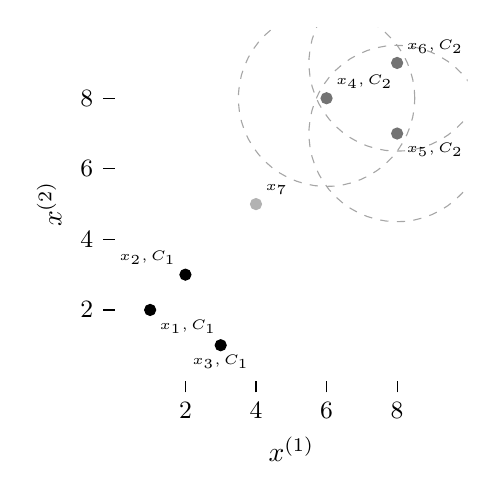
\begin{tikzpicture}
    \begin{axis}[
        xlabel={$x^{(1)}$}, ylabel={$x^{(2)}$},
        xmin=0, xmax=10, ymin=0, ymax=10,
        width=0.5\textwidth, height=0.5\textwidth,
        axis line style={draw=none},
        tick style={black, thin},
        xtick={2,4,6,8}, ytick={2,4,6,8},
        xticklabel style={font=\small},
        yticklabel style={font=\small},
        tick align=outside, tick pos=left,
    ]
    \addplot[black!35, dashed, thin, domain=0:360, samples=60]
        ({6 + 2.5*cos(x)}, {8 + 2.5*sin(x)});
    \addplot[black!35, dashed, thin, domain=0:360, samples=60]
        ({8 + 2.5*cos(x)}, {7 + 2.5*sin(x)});
    \addplot[black!35, dashed, thin, domain=0:360, samples=60]
        ({8 + 2.5*cos(x)}, {9 + 2.5*sin(x)});
    % C1 sealed (dark)
    \addplot[only marks, mark=*, mark size=2pt, black]
        coordinates {(1,2)(2,3)(3,1)};
    % C2 forming (grey)
    \addplot[only marks, mark=*, mark size=2pt, black!55]
        coordinates {(6,8)(8,7)(8,9)};
    % x7 still unvisited
    \addplot[only marks, mark=*, mark size=2pt, black!30]
        coordinates {(4,5)};
    \node[font=\tiny, anchor=north west] at (axis cs:1,2) {$x_1, C_1$};
    \node[font=\tiny, anchor=south east] at (axis cs:2,3) {$x_2, C_1$};
    \node[font=\tiny, anchor=north]      at (axis cs:3,1) {$x_3, C_1$};
    \node[font=\tiny, anchor=south west] at (axis cs:6,8) {$x_4, C_2$};
    \node[font=\tiny, anchor=north west] at (axis cs:8,7) {$x_5, C_2$};
    \node[font=\tiny, anchor=south west] at (axis cs:8,9) {$x_6, C_2$};
    \node[font=\tiny, anchor=south west] at (axis cs:4,5) {$x_7$};
    \end{axis}
\end{tikzpicture}
\caption{\newthought{Visit $x_4$}: $N_{2.5}(x_4){=}\{x_4,\,x_5,\,x_6\}$, $|N|{=}3 \geq 2$, so $x_4$ is core. Seed $C_2$; expand from $x_5$ and $x_6$: both are core and their neighbourhoods cover only $\{x_4,x_5,x_6\}$. $C_2{=}\{x_4,\,x_5,\,x_6\}$ sealed. Only $x_7$ remains unvisited.}
\label{fig:dbscan_trace_c2}
\end{figure}


\begin{figure}
\centering
\begin{tikzpicture}
    \begin{axis}[
        xlabel={$x^{(1)}$}, ylabel={$x^{(2)}$},
        xmin=0, xmax=10, ymin=0, ymax=10,
        width=0.5\textwidth, height=0.5\textwidth,
        axis line style={draw=none},
        tick style={black, thin},
        xtick={2,4,6,8}, ytick={2,4,6,8},
        xticklabel style={font=\small},
        yticklabel style={font=\small},
        tick align=outside, tick pos=left,
    ]
    \addplot[black!30, dashed, thin, domain=0:360, samples=60]
        ({4 + 2.5*cos(x)}, {5 + 2.5*sin(x)});
    % C1 sealed (dark)
    \addplot[only marks, mark=*, mark size=2pt, black]
        coordinates {(1,2)(2,3)(3,1)};
    % C2 sealed (grey)
    \addplot[only marks, mark=*, mark size=2pt, black!55]
        coordinates {(6,8)(8,7)(8,9)};
    % x7 noise (open circle)
    \addplot[only marks, mark=o, mark size=3pt, black, thick]
        coordinates {(4,5)};
    \node[font=\tiny, anchor=north west] at (axis cs:1,2) {$x_1, C_1$};
    \node[font=\tiny, anchor=south east] at (axis cs:2,3) {$x_2, C_1$};
    \node[font=\tiny, anchor=north]      at (axis cs:3,1) {$x_3, C_1$};
    \node[font=\tiny, anchor=south west] at (axis cs:6,8) {$x_4, C_2$};
    \node[font=\tiny, anchor=north west] at (axis cs:8,7) {$x_5, C_2$};
    \node[font=\tiny, anchor=south west] at (axis cs:8,9) {$x_6, C_2$};
    \node[font=\tiny, anchor=south west] at (axis cs:4,5) {$x_7, \text{noise}$};
    \end{axis}
\end{tikzpicture}
\caption{\newthought{Visit $x_7$}: $N_{2.5}(x_7){=}\{x_7\}$, $|N|{=}1 < 2$, so $x_7$ is noise. The dashed circle is empty; no neighbour lies within $\varepsilon{=}2.5$. All points visited. Final result: $C_1{=}\{x_1,x_2,x_3\}$ (dark), $C_2{=}\{x_4,x_5,x_6\}$ (grey), noise$\,{=}\{x_7\}$ (open circle). No value of $K$ was chosen; noise was never forced into a cluster.}
\label{fig:dbscan_trace_noise}
\end{figure}

\marginnote[-12em]{%
\begin{align*}
    d(x_7,\,x_3) &= \sqrt{1+16} = \sqrt{17} \approx 4.12 \;\times \\
    d(x_7,\,x_4) &= \sqrt{4+9}  = \sqrt{13} \approx 3.61 \;\times
\end{align*}%
The nearest candidates are both outside $\varepsilon$.%
}

\vspace{2.5em}

\newthought{Parameter Selection}\index{DBSCAN!parameter selection}

\newthought{Choosing $\mathrm{minPts}$} follows a practical rule of thumb: set $\mathrm{minPts} \geq d{+}1$ where $d$ is the number of dimensions.
For two-dimensional data, $\mathrm{minPts}{=}3$ or $4$ is typical; higher dimensions require larger values to avoid sparse neighbourhoods being treated as dense.

\newthought{Choosing $\varepsilon$} uses the $k$-distance plot\index{k-distance plot}: for each point, compute the distance to its $k$-th nearest neighbour (with $k{=}\mathrm{minPts}{-}1$) and sort these distances in ascending order.
The curve rises slowly in dense regions and sharply in sparse ones; the elbow of the curve is the recommended $\varepsilon$.

\begin{marginfigure}
\centering
\begin{tikzpicture}
    \begin{axis}[
        xlabel={Points (sorted)},
        ylabel={$k$-distance},
        xmin=0, xmax=100,
        ymin=0, ymax=2,
        width=\marginparwidth,
        height=\marginparwidth,
        axis line style={draw=none},
        tick style={black, thin},
        xtick={0,50,100},
        ytick={0,1,2},
        xticklabel style={font=\tiny},
        yticklabel style={font=\tiny},
        tick align=outside,
        tick pos=left,
    ]
    \addplot[black, thick, smooth] coordinates {
        (0,0.10)(20,0.15)(40,0.20)(60,0.30)(70,0.50)(80,1.00)(90,1.50)(100,1.80)
    };
    \draw[black!50, dashed] (axis cs:0,0.5) -- (axis cs:100,0.5);
    \node[font=\tiny, anchor=west] at (axis cs:48,0.65) {$\varepsilon{\approx}0.5$};
    \end{axis}
\end{tikzpicture}
\caption{$k$-distance plot. The elbow at ${\approx}0.5$ marks the transition from dense to sparse regions.}
\label{fig:kdistance_plot}
\end{marginfigure}


\newthought{Failure Modes of DBSCAN}\index{failure modes!DBSCAN}

\newthought{DBSCAN has its own pathologies.}
The two most common arise from the single global $\varepsilon$ and from high-dimensional spaces.

\vspace{2.5em}
\marginnote{\newthought{Varying density}}

\begin{figure}
\centering
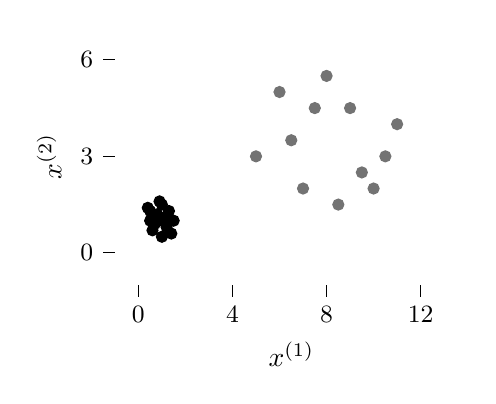
\begin{tikzpicture}
    \begin{axis}[
        xlabel={$x^{(1)}$}, ylabel={$x^{(2)}$},
        xmin=-1, xmax=14, ymin=-1, ymax=7,
        width=0.5\textwidth, height=0.4\textwidth,
        axis line style={draw=none},
        tick style={black, thin},
        xtick={0,4,8,12}, ytick={0,3,6},
        xticklabel style={font=\small},
        yticklabel style={font=\small},
        tick align=outside, tick pos=left,
    ]
    % Tight, dense cluster (small epsilon needed)
    \addplot[only marks, mark=*, mark size=2pt, black] coordinates {
        (0.5,1.0)(1.0,0.5)(1.0,1.5)(1.5,1.0)(0.8,1.2)
        (0.6,0.7)(1.2,0.8)(1.3,1.3)(0.9,1.6)(0.4,1.4)
        (1.1,1.1)(0.7,0.9)(1.4,0.6)(0.5,1.3)(1.0,1.0)
    };
    % Spread, sparse cluster (large epsilon needed)
    \addplot[only marks, mark=*, mark size=2pt, black!55] coordinates {
        (5.0,3.0)(7.0,2.0)(9.0,4.5)(8.5,1.5)(6.0,5.0)(10.5,3.0)
        (11.0,4.0)(6.5,3.5)(8.0,5.5)(10.0,2.0)(7.5,4.5)(9.5,2.5)
    };
    \end{axis}
\end{tikzpicture}
\caption{Varying cluster density. An $\varepsilon$ tight enough to resolve the left cluster will leave the right cluster disconnected; an $\varepsilon$ large enough to connect the right cluster will merge everything on the left into one blob.}
\label{fig:dbscan_fail_density}
\end{figure}

\marginnote{\newthought{OPTICS}\index{OPTICS} (Ordering Points To Identify the Clustering Structure) addresses varying density by assigning each point a reachability distance: $\mathrm{reach}(p,\,o) = \max(\mathrm{core\text{-}dist}(o),\; d(o,p))$, where core-dist is the distance to the $\mathrm{minPts}$-th nearest neighbour of $o$. Plotting sorted reachability values produces valleys (dense clusters) and peaks (sparse separations) at every scale simultaneously, removing the need for a single global $\varepsilon$.}

\newthought{High dimensionality}\index{curse of dimensionality} degrades DBSCAN because all pairwise distances converge as $d$ grows: the ratio of maximum to minimum distance approaches 1, making $\varepsilon$-neighbourhoods either empty or the entire dataset.
In practice, DBSCAN is most reliable in two to twenty dimensions.

\newthought{When DBSCAN struggles,} the root cause is always the same: density is a global threshold applied uniformly across a space that may not be uniform.
The remedy is either to adapt the threshold locally (OPTICS) or to abandon distance metrics in favour of graph connectivity (spectral clustering).

\marginnote{\newthought{HDBSCAN}\index{HDBSCAN} (Hierarchical DBSCAN) takes this further: it sweeps $\varepsilon$ from $\infty$ down to $0$, building a hierarchy of all density-based clusterings at once, then extracts the most persistent clusters automatically. No single $\varepsilon$ is ever chosen. The result combines the multi-scale view of hierarchical clustering with DBSCAN's ability to handle noise and arbitrary shapes.}


\vspace{2.5em}

\newthought{Spectral Clustering}\index{spectral clustering}

\newthought{Spectral clustering}\index{spectral clustering} transforms the data into a graph and finds clusters as well-separated subgraphs.
It works even when clusters are non-convex, because connectivity rather than geometric proximity determines membership.

\newthought{The similarity graph}\index{similarity graph} is built by computing a weight $w_{ij}$ for every pair of points.
The most common choice is the Gaussian kernel:
\begin{align*}
    w_{ij} &= \exp\!\left(-\frac{\|x_i - x_j\|^2}{2\sigma^2}\right)
\end{align*}

Points that are close receive weight near 1; distant points receive weight near 0.
The bandwidth $\sigma$ controls how quickly similarity falls off with distance.

\newthought{The graph Laplacian}\index{graph Laplacian} encodes the graph's connectivity in matrix form.
Let $W$ be the $n \times n$ weight matrix and $D$ the diagonal degree matrix with $D_{ii} = \sum_j w_{ij}$.
The unnormalized Laplacian is:
\begin{align*}
    L &= D - W
\end{align*}

The normalized Laplacian, which corrects for differences in node degree, is:
\begin{align*}
    L_{\mathrm{sym}} &= D^{-1/2}\, L\, D^{-1/2} \\
                     &= I - D^{-1/2}\, W\, D^{-1/2}
\end{align*}

\marginnote{\newthought{Why eigenvectors?} The number of zero eigenvalues of $L$ equals the number of connected components. The $k$ smallest eigenvectors embed the data so that points in the same component land nearby; K-Means in this embedding finds well-separated clusters even when the original space is non-convex.}

\newthought{The algorithm} computes the $k$ smallest eigenvectors of $L_{\mathrm{sym}}$, stacks them as columns into a matrix $U \in \mathbb{R}^{n \times k}$, normalises each row of $U$ to unit length, and runs K-Means on the rows.

\begin{figure}
\centering
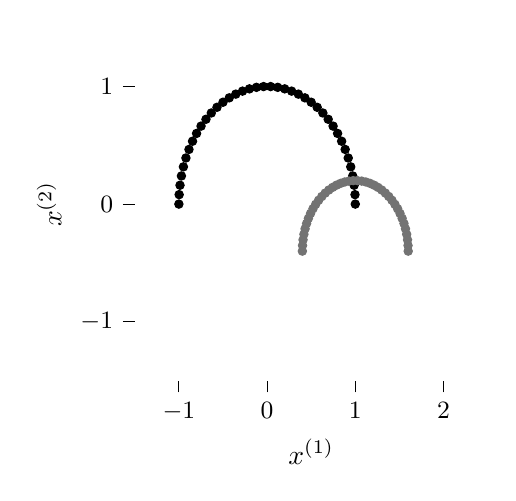
\begin{tikzpicture}
    \begin{axis}[
        xlabel={$x^{(1)}$}, ylabel={$x^{(2)}$},
        xmin=-1.5, xmax=2.5, ymin=-1.5, ymax=1.5,
        width=0.5\textwidth, height=0.5\textwidth,
        axis line style={draw=none},
        tick style={black, thin},
        xtick={-1,0,1,2}, ytick={-1,0,1},
        xticklabel style={font=\small},
        yticklabel style={font=\small},
        tick align=outside, tick pos=left,
    ]
    \addplot[only marks, mark=*, mark size=1.5pt, black,
        domain=0:180, samples=40] ({cos(x)}, {sin(x)});
    \addplot[only marks, mark=*, mark size=1.5pt, black!55,
        domain=0:180, samples=40] ({1+0.6*cos(x)}, {-0.4+0.6*sin(x)});
    \end{axis}
\end{tikzpicture}
\caption{Two interlocking crescents in the original feature space. The clusters are non-convex and inseparable by any straight boundary. No centroid-based method can recover both groups.}
\label{fig:spectral_original}
\end{figure}

\begin{figure}
\centering
\begin{tikzpicture}
    \begin{axis}[
        xlabel={$v_1$}, ylabel={$v_2$},
        xmin=-0.25, xmax=0.25, ymin=-0.25, ymax=0.25,
        width=0.5\textwidth, height=0.5\textwidth,
        axis line style={draw=none},
        tick style={black, thin},
        xtick={-0.2,0,0.2}, ytick={-0.2,0,0.2},
        xticklabel style={font=\small},
        yticklabel style={font=\small},
        tick align=outside, tick pos=left,
    ]
    \addplot[only marks, mark=*, mark size=1.5pt, black] coordinates {
        (-0.15, 0.10)(-0.14, 0.08)(-0.13, 0.09)
        (-0.12, 0.07)(-0.16, 0.11)(-0.11, 0.08)
        (-0.17, 0.09)(-0.10, 0.10)(-0.13, 0.12)
        (-0.14, 0.06)(-0.12, 0.11)(-0.15, 0.07)
        (-0.11, 0.09)(-0.16, 0.08)(-0.13, 0.10)
    };
    \addplot[only marks, mark=*, mark size=1.5pt, black!55] coordinates {
        ( 0.15,-0.10)( 0.14,-0.08)( 0.13,-0.09)
        ( 0.12,-0.07)( 0.16,-0.11)( 0.11,-0.08)
        ( 0.17,-0.09)( 0.10,-0.10)( 0.13,-0.12)
        ( 0.14,-0.06)( 0.12,-0.11)( 0.15,-0.07)
        ( 0.11,-0.09)( 0.16,-0.08)( 0.13,-0.10)
    };
    \end{axis}
\end{tikzpicture}
\caption{After embedding into the two leading eigenvectors of $L_{\mathrm{sym}}$, the same crescents from Figure~\ref{fig:spectral_original} are linearly separable and K-Means succeeds.}
\label{fig:spectral_embedding}
\end{figure}

\vspace{2.5em}

\newthought{Computational Complexity}\index{computational complexity!density clustering}

\marginnote{\newthought{Mean Shift}\index{mean shift} is a mode-seeking algorithm: each point iteratively moves to the weighted mean of its neighbourhood under a kernel $K$ with bandwidth $h$. Points converging to the same mode form a cluster. It requires no $K$ and finds non-convex clusters, but the bandwidth $h$ plays the same role as $\varepsilon$ and the $O(n^2)$ per-iteration cost limits it to moderate $n$.}

\begin{table*}[ht]
\centering
\begin{tabular}{p{0.26\textwidth}p{0.12\textwidth}p{0.12\textwidth}p{0.34\textwidth}}
    \toprule
    \textbf{Algorithm} & \textbf{Time} & \textbf{Space} & \textbf{Notes} \\
    \midrule
    K-Means (baseline)  & $O(nKTd)$    & $O(n{+}K)$ & $K$ and $T$ chosen in advance; no noise concept; fails on non-convex clusters \\
    DBSCAN (naive)      & $O(n^2)$     & $O(n^2)$ & $O(n \log n)$ with k-d tree or ball tree in low dimensions \\
    OPTICS              & $O(n^2)$     & $O(n)$   & No fixed $\varepsilon$; produces full reachability ordering \\
    Mean Shift          & $O(n^2 T)$   & $O(n)$   & $T$ iterations; exact cluster count unknown until convergence \\
    Spectral clustering & $O(n^3)$     & $O(n^2)$ & Eigendecomposition dominates; sparse graph approximations reduce cost \\
    \bottomrule
\end{tabular}
\vspace{2em}
\caption{Computational complexity of density and graph-based clustering methods, with K-Means listed as a baseline. DBSCAN with a spatial index is practical for large $n$ in low dimensions. Spectral clustering is prohibitive for large $n$ without sparse graph approximations.}
\label{tab:density_complexity}
\end{table*}

\newthought{The similarity matrix} in spectral clustering is the dominant bottleneck.
Storing all $\tfrac{n(n-1)}{2}$ pairwise weights requires $O(n^2)$ memory, and the eigendecomposition of the $n \times n$ Laplacian costs $O(n^3)$.
Practical implementations use sparse graphs (connecting each point to only its $k$ nearest neighbours) to reduce both costs substantially.


% ==============================================================================================
% BLOCK 3: STUDENT ACTIVATION
% ==============================================================================================

\newpage

\section{Examples \& Exercises}\index{examples}\index{exercises}

\newthought{Computing by hand} reveals what the algorithm actually does at each step; run it slowly and feel where density propagates and where it stops.

\vspace{1em}

\begin{marginfigure}
    \centering
    \begin{tikzpicture}
        \begin{axis}[
            xmin=0, xmax=10,
            ymin=0, ymax=10,
            width=\marginparwidth,
            height=\marginparwidth,
            axis line style={draw=none},
            tick style={black, thin},
            xtick={0,3,6,9},
            ytick={0,3,6,9},
            xticklabel style={font=\tiny},
            yticklabel style={font=\tiny},
            tick align=outside,
            tick pos=left,
            xlabel={$x^{(1)}$},
            ylabel={$x^{(2)}$},
        ]
        \addplot[only marks, mark=*, mark size=2pt, black]    coordinates {(1,2)(2,3)(3,1)};
        \addplot[only marks, mark=*, mark size=2pt, black!55] coordinates {(6,8)(8,7)(8,9)};
        \addplot[only marks, mark=*, mark size=2pt, black!30] coordinates {(4,5)};
        \node[font=\tiny, anchor=south east] at (axis cs:1,2) {$x_1$};
        \node[font=\tiny, anchor=south east] at (axis cs:2,3) {$x_2$};
        \node[font=\tiny, anchor=north]      at (axis cs:3,1) {$x_3$};
        \node[font=\tiny, anchor=south west] at (axis cs:6,8) {$x_4$};
        \node[font=\tiny, anchor=north west] at (axis cs:8,7) {$x_5$};
        \node[font=\tiny, anchor=south west] at (axis cs:8,9) {$x_6$};
        \node[font=\tiny, anchor=south west] at (axis cs:4,5) {$x_7$};
        \end{axis}
    \end{tikzpicture}
    \caption{Seven points for the DBSCAN trace. $x_7{=}(4,5)$ sits between the two natural groups.}
    \label{fig:dbscan_exercise_scatter}
\end{marginfigure}

\newthought{Given seven points} $x_1{=}(1,2)$, $x_2{=}(2,3)$, $x_3{=}(3,1)$, $x_4{=}(6,8)$, $x_5{=}(8,7)$, $x_6{=}(8,9)$, $x_7{=}(4,5)$, run DBSCAN with $\varepsilon{=}2.5$ and $\mathrm{minPts}{=}2$.
Your tasks: compute the neighbourhood size $|N_{2.5}(x_i)|$ for each point, classify each point as core, border, or noise, and identify the clusters.

\vspace{0.5em}

\newthought{Neighbourhood sizes.} For each point $x_i$ count all points within distance 2.5 (including $x_i$ itself).
Here is the full calculation for $x_1$:

\begin{align*}
    d(x_1,\,x_2) &= \sqrt{(2-1)^2 + (3-2)^2} \\
                 &= \sqrt{1 + 1} \\
                 &= \sqrt{2} \\
                 &\approx 1.41 \quad (\leq 2.5,\; \text{counted}) \\[4pt]
    d(x_1,\,x_3) &= \sqrt{(3-1)^2 + (1-2)^2} \\
                 &= \sqrt{4 + 1} \\
                 &= \sqrt{5} \\
                 &\approx 2.24 \quad (\leq 2.5,\; \text{counted}) \\[4pt]
    d(x_1,\,x_7) &= \sqrt{(4-1)^2 + (5-2)^2} \\
                 &= \sqrt{9 + 9} \\
                 &= \sqrt{18} \\
                 &\approx 4.24 \quad (> 2.5,\; \text{not counted})
\end{align*}

So $N_{2.5}(x_1) = \{x_1,\, x_2,\, x_3\}$ and $|N_{2.5}(x_1)| = 3 \geq 2$: $x_1$ is a \textbf{core point}.
Compute the remaining neighbourhood sizes yourself, then verify against the table below.

\vspace{2.5em}

\begin{table*}[ht]
\centering
\begin{tabular}{p{0.07\textwidth}p{0.12\textwidth}p{0.10\textwidth}p{0.12\textwidth}p{0.30\textwidth}p{0.10\textwidth}}
    \toprule
    \textbf{Point} & \textbf{Coords} & \textbf{$|N_{2.5}|$} & \textbf{Type} & \textbf{Neighbours in $N_{2.5}$} & \textbf{Cluster} \\
    \midrule
    $x_1$ & $(1,2)$ & $3$ & Core  & $\{x_1,\, x_2,\, x_3\}$          & $C_1$ \\
    $x_2$ & $(2,3)$ & $3$ & Core  & $\{x_1,\, x_2,\, x_3\}$          & $C_1$ \\
    $x_3$ & $(3,1)$ & $3$ & Core  & $\{x_1,\, x_2,\, x_3\}$          & $C_1$ \\
    $x_4$ & $(6,8)$ & $3$ & Core  & $\{x_4,\, x_5,\, x_6\}$          & $C_2$ \\
    $x_5$ & $(8,7)$ & $3$ & Core  & $\{x_4,\, x_5,\, x_6\}$          & $C_2$ \\
    $x_6$ & $(8,9)$ & $3$ & Core  & $\{x_4,\, x_5,\, x_6\}$          & $C_2$ \\
    $x_7$ & $(4,5)$ & $1$ & Noise & $\{x_7\}$ only                    & $-$ \\
    \bottomrule
\end{tabular}
\vspace{2em}
\caption{DBSCAN trace for $\varepsilon{=}2.5$, $\mathrm{minPts}{=}2$. All six canonical points are core points; $x_7$ has no neighbour within radius 2.5 and is labelled noise. The two natural clusters are recovered without specifying $K$ and without assigning the noise point to either group.}
\label{tab:dbscan_trace}
\end{table*}

\newthought{Verify $x_7$ is noise.} Compute $d(x_7,\,x_3)$ to confirm that $x_7$ lies outside the $\varepsilon$-neighbourhood of its nearest candidate:
\begin{align*}
    d(x_7,\,x_3) &= \sqrt{(4-3)^2 + (5-1)^2} \\
                 &= \sqrt{1 + 16} \\
                 &= \sqrt{17} \\
                 &\approx 4.12 \quad (> 2.5)
\end{align*}
Compute $d(x_7,\,x_4)$ yourself.
Why is $x_7$ correctly identified as noise rather than being assigned to whichever cluster is nearer?

\newpage

\newthought{Parameter sensitivity.} Re-run the trace with $\varepsilon{=}4.5$ and $\mathrm{minPts}{=}2$.
Does $x_7$ change classification?
At what minimum value of $\varepsilon$ does $x_7$ first enter the neighbourhood of some core point?

\newthought{Comparison with K-Means.} Run K-Means with $K{=}2$ on the same seven points.
Which cluster does K-Means assign $x_7$ to?
Is that assignment more or less informative than DBSCAN's noise label, and why?

\newthought{K-Means baseline result.} After convergence with $K{=}2$, the centroids settle at $\mu_1 \approx (2.0,\,2.0)$ and $\mu_2 \approx (7.3,\,8.0)$.
Point $x_7{=}(4,5)$ is closer to $\mu_1$:
\begin{align*}
    d(x_7,\,\mu_1) &= \sqrt{(4-2)^2 + (5-2)^2} \\
                   &= \sqrt{4+9} \\
                   &= \sqrt{13} \approx 3.61 \\[4pt]
    d(x_7,\,\mu_2) &= \sqrt{(4-7.3)^2 + (5-8.0)^2} \\
                   &= \sqrt{10.89+9} \\
                   &= \sqrt{19.89} \approx 4.46
\end{align*}
K-Means assigns $x_7$ to $C_1$, as shown below.
The assignment is not wrong in a strict sense; it is simply forced.
K-Means has no noise concept and cannot abstain.

\begin{figure}
\centering
\begin{tikzpicture}
    \begin{axis}[
        xlabel={$x^{(1)}$}, ylabel={$x^{(2)}$},
        xmin=0, xmax=10, ymin=0, ymax=10,
        width=0.5\textwidth, height=0.5\textwidth,
        axis line style={draw=none},
        tick style={black, thin},
        xtick={2,4,6,8}, ytick={2,4,6,8},
        xticklabel style={font=\small},
        yticklabel style={font=\small},
        tick align=outside, tick pos=left,
    ]
    % C1 points (dark) including x7
    \addplot[only marks, mark=*, mark size=2pt, black]
        coordinates {(1,2)(2,3)(3,1)(4,5)};
    % C1 centroid
    \addplot[only marks, mark=+, mark size=5pt, black, thick]
        coordinates {(2.5,2.75)};
    % C2 points (grey)
    \addplot[only marks, mark=*, mark size=2pt, black!55]
        coordinates {(6,8)(8,7)(8,9)};
    % C2 centroid
    \addplot[only marks, mark=+, mark size=5pt, black!55, thick]
        coordinates {(7.33,8)};
    % Labels
    \node[font=\tiny, anchor=north west] at (axis cs:1,2)   {$x_1$};
    \node[font=\tiny, anchor=south east] at (axis cs:2,3)   {$x_2$};
    \node[font=\tiny, anchor=north]      at (axis cs:3,1)   {$x_3$};
    \node[font=\tiny, anchor=south west] at (axis cs:4,5)   {$x_7$};
    \node[font=\tiny, anchor=south west] at (axis cs:6,8)   {$x_4$};
    \node[font=\tiny, anchor=north west] at (axis cs:8,7)   {$x_5$};
    \node[font=\tiny, anchor=south west] at (axis cs:8,9)   {$x_6$};
    \node[font=\tiny, anchor=south east] at (axis cs:2.5,2.75) {$\mu_1$};
    \node[font=\tiny, anchor=south west] at (axis cs:7.33,8)   {$\mu_2$};
    \end{axis}
\end{tikzpicture}
\caption{K-Means baseline with $K{=}2$. Crosses mark centroids $\mu_1$ and $\mu_2$. Because K-Means must assign every point, $x_7$ is forced into $C_1$ (dark). Compare with Figure~\ref{fig:dbscan_trace_noise}: DBSCAN labels $x_7$ noise and makes no forced assignment.}
\label{fig:kmeans_baseline}
\end{figure}

\marginnote{\newthought{Code} will be provided as a Python notebook.}

\newthought{A geospatial dataset to explore.} Apply DBSCAN to a set of GPS coordinates (e.g., city check-in records or taxi pickup points).

\newthought{What to observe.}
Try several $(\varepsilon, \mathrm{minPts})$ combinations and note how the number of clusters and noise points change.
Plot the $k$-distance curve before choosing $\varepsilon$, and check whether the elbow matches the value that gives the most interpretable clustering.


\section{Self-Reflection and Recap}\index{reflection}\index{recap}

\newthought{Self-Reflection} questions to guide your thinking:
\begin{itemize}
    \item Why can DBSCAN find clusters of arbitrary shape while K-Means cannot?
    \item What happens to a border point if $\mathrm{minPts}$ is increased by one?
    \item Why is density reachability not symmetric, and what does that asymmetry imply for cluster assignment?
    \item DBSCAN with a very large $\varepsilon$ and $\mathrm{minPts}{=}1$ behaves like which simpler algorithm?
    \item OPTICS removes the need for a fixed $\varepsilon$; what does it require from the user instead?
    \item In what sense does spectral clustering use K-Means internally, and why is that not a contradiction?
    \item Why does the number of zero eigenvalues of the Laplacian reveal the number of connected components?
    \item When would you prefer DBSCAN over hierarchical clustering, even if both recover the correct partition?
\end{itemize}

\newthought{Recap} of Key Concepts:
\begin{itemize}
    \item \textbf{DBSCAN} classifies every point as core, border, or noise using $\varepsilon$ and $\mathrm{minPts}$, and builds clusters by propagating density reachability from core points outward without specifying $K$.
    \item \textbf{Noise handling} is native: any point with fewer than $\mathrm{minPts}$ neighbours within $\varepsilon$ is labelled noise and excluded from all clusters.
    \item \textbf{OPTICS} removes the single global $\varepsilon$ by producing a reachability plot that exposes cluster structure at every density scale simultaneously.
    \item \textbf{Spectral clustering} embeds data into the eigenvectors of the graph Laplacian, making non-convex clusters linearly separable before applying K-Means.
    \item \textbf{Parameter sensitivity} is the shared weakness: $\varepsilon$ and $\sigma$ must be chosen carefully, and both methods degrade in high dimensions where all distances become indistinguishable.
\end{itemize}

\marginnote{\newthought{The root of density failure.} Every density-based method sets a single threshold on what counts as close enough. When true cluster density varies across the dataset, no fixed value works everywhere.}

\newthought{Density-based and graph-based methods} both escape the spherical cluster assumption, but they still operate in the original feature space.
With ten features the $\varepsilon$-ball captures something meaningful; with a thousand features it either captures everything or nothing.
The same data that breaks DBSCAN in high dimensions also makes the similarity graph in spectral clustering nearly uniform, erasing the connectivity structure that the eigenvectors are supposed to encode.

\newthought{The underlying problem} is that the data occupies a high-dimensional space but the meaningful variation lives in far fewer dimensions.
Before we can cluster reliably at scale, we need to find those dimensions.

\marginnote{\newthought{Teaser} If cluster structure lives in a low-dimensional subspace, can we find that subspace without knowing the clusters first? And can we do it in a way that preserves the global geometry, the local geometry, or both?}
